\documentclass{article}
\usepackage{amsmath,amssymb,graphicx}
\usepackage{hyperref}
\title{CSC236 Winter 2015, Assignment 3}
\author{Connor Peet}
\renewcommand{\today}{~}
\hypersetup{pdfpagemode=Fullscreen,
  colorlinks=true,
  linkfileprefix={}}
\newcommand{\floor}[1]{\lfloor #1\rfloor}
\begin{document}
\maketitle

\begin{figure}[p]
    \centering
    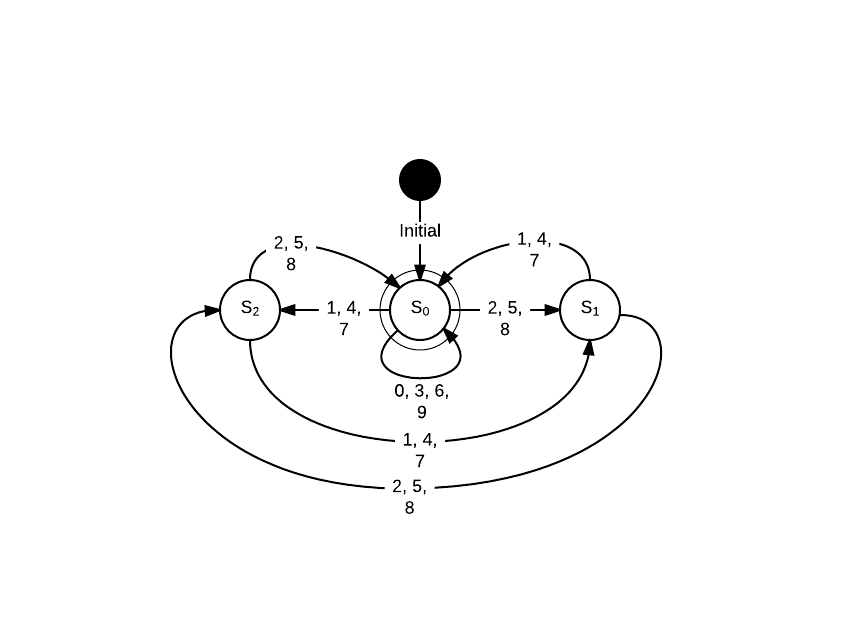
\includegraphics[width=\textwidth]{a3q1}
    \caption{A small DFA that accepts natural numbers which are multiples of three.}
    \label{fig:awesome_image}
\end{figure}

\begin{enumerate}

\item
    The DFA designed can be seen in figure~\ref{fig:awesome_image}. It has three states: $S_0$, $S_1$, and $S_2$. I will prove by contradiction that that is the minimum number of states required to fit the specification given in Question 1.

    Suppose we only have two states, and have some strings strings $w_1 = 2, w_2 = 24, w_3 = 242$. According to the specification, the empty string is accepted, so the initial state is accepting, and the other state must not accept. (Otherwise we'd just take any string, and that doesn't clearly work!) Therefore:

        \begin{itemize}
        \item $w_1$ must transition to the non-accepting state on $2$, since $2$ is not divisible by three.
        \item $w_2$ transitions to non-accepting on $2$ and accepting on $4$, since $24$ is divisible by three.
        \item $w_3$ transitions to non-accepting on $2$, accepting on $4$, and stays in accepting on $2$.
        \end{itemize}

    The third and first cases contradict each other, since $w_1$ requires $2$ to transition \textit{out of} the accepting state, and $w_3$ requires $2$ to transition \textit{into} the accepting state.

    Therefore, in order to build a DFA to specific we require at least three states.

\end{enumerate}

\end{document}
